\documentclass[10pt,a4paper]{article}
\usepackage[utf8]{inputenc}
\usepackage[german]{babel}
\usepackage[T1]{fontenc}
\usepackage{graphicx}
\usepackage[paper=a4paper,width=14cm,left=35mm,height=22cm]{geometry}
\usepackage{setspace}
\usepackage{charter}
\usepackage{subfig}
\linespread{1.15}
\setlength{\parskip}{0.25em}
\setlength{\parindent}{0em}

\usepackage{color}
\usepackage{listings}
\lstset{
	basicstyle=\sffamily, 
	columns=[l]flexible, 
	mathescape=true, 
  	showstringspaces=false, 
  	numbers=left, 
  	numberstyle=\tiny,
  	keywordstyle=\color[rgb]{0,0,1},
    commentstyle=\color[rgb]{0.133,0.545,0.133},
    stringstyle=\color[rgb]{0.627,0.126,0.941},
}
\lstset{language=java}
\usepackage{float}
\newfloat{listing}{htbp}{scl}[section]
\floatname{listing}{Listing}

\usepackage{wrapfig}

\usepackage[usenames,dvipsnames]{xcolor}
\usepackage{hyperref}
\hypersetup{
    bookmarks=true,
    colorlinks=true,
    linkcolor=NavyBlue,
    citecolor=NavyBlue,
    urlcolor=NavyBlue
}

\usepackage{amsfonts}

\begin{document}
\author{Coralie Reuter und Markus Tacker}
\title{\emph{GroupMood}: Mobile Anwendung zur schnellen Erfassung und Auswertung von Stimmungen und Meinungen in einer Gruppe.}
\begin{center}

\includegraphics[width=10cm]{media/GroupMood.png}

\begin{huge}GroupMood\end{huge}

\begin{large}Mobile Anwendung zur schnellen Erfassung und Auswertung von Stimmungen und Meinungen in einer Gruppe\end{large}

Coralie Reuter und Markus Tacker

\today

\end{center}

\bigskip 

\section*{Zusammenfassung}

\emph{GroupMood} ermöglich es, eine Gruppe von Personen schnell und direkt mit Hilfe ihres Smartphones zu befragen. Da Smartphones inzwischen weit verbreitet sind, werden diese mit Hilfe der App als interaktiver Rückkanal verwendet. Die Anwendung ermöglicht es den Teilnehmern, im Verlauf einer Veranstaltung an Umfragen teilzunehmen oder Kommentare abzugeben. Im ersten Abschnitt wird die grundlegende Idee und das Konzept der Gruppenbefragungen vorgestellt, in dem erläutert wird, welche Arten von Fragen im Verlauf einer Veranstaltung auftreten. Im zweiten Abschnitt wird die Umsetzung der Idee beschrieben, deren Konzept dabei so flexibel ist, das beliebige Arten von Veranstaltungen integriert werden können und darüber hinaus weitere Anwendungsmöglichkeiten denkbar sind.


\tableofcontents

\section{Einleitung}

Heutzutage ist es üblich, dass Präsentation durch Teilnehmer bewertet werden. Dieses Feedback wird entweder durch Fragebögen oder mit Hilfe von browserbasierten Anwendungen wie z.B. \emph{joind.in}\footnote{\url{http://joind.in/}} nach einer Präsentation erfasst. Hierbei bewerten die Teilnehmer die Präsentation sowohl im Hinblick auf die didaktische Aufbereitung als auch auf "`weiche"' Faktoren wie z.B. das persönliche Auftreten des Präsentierenden. Diese Bewertung spiegelt immer den subjektiven Eindruck der Teilnehmer über den Verlauf der gesamten Präsentation wieder -- eine individuelle Bewertung einzelner Folien ist dabei nicht möglich. Um bessere und genauere Bewertungen zu erhalten, müssten diese idealerweise schon im Laufe einer Präsentation abgegeben werden können. Es fehlt also ein direkter, verzögerungsfreier Kanal um Bewertungen einer Präsentation durch deren Teilnehmer zu erfassen.

Feedback muss dabei nicht auf die Bewertung einer Veranstaltung beschränkt sein. Eine interaktive Beteiligung durchbricht den üblichen Ablauf von Präsentation, bei denen eine Person vorträgt und alle anderen passiv zuhören. So kann man eine bessere Aufnahme des Themas bei den Teilnehmern erreichen. Beispiel hierfür sind Aufgaben, die von den Teilnehmern durch Auswählen einer Antwort gelöst werden, und bei denen anschließend die Ergebnisse aller Teilnehmer gemittelt dargestellt werden. Diese Art von Interaktion dient zur schnellen Kontrolle des Wissensstandes für den einzelnen, liefert aber auch dem Lehrenden einen schnellen und direkten Überblick über den Leistungsstand der Teilnehmer. Hierfür existieren schon Systeme wie \emph{QuizDom}\footnote{\url{http://www.qwizdom.com/}}, bei denen Klassenraum-Ausstattungen aber leicht mehrere tausend Euro kosten \footnote{\url{http://www.dreamav.co.uk/qwizdom_q4.html}}. Mit diesen Geräten können die Teilnehmer, nachdem die Geräte an jeden einzelnen ausgeteilt wurden, Fragen mithilfe der Tastatur auf den Geräten beantworten, die dann unmittelbar ausgewertet werden können. Ein direkter Rückkanal zum Teilnehmer existiert aber hierbei nicht.

\section{Gruppenbefragung}

Gerade bei jüngeren Personen und im Business-Umfeld sind SmartPhones inzwischen sehr weit verbreitet -- \emph{GroupMood} schafft für Teilnehmer die Möglichkeit, Veranstaltungen jeder Art auf dem eigenen mobilen Endgerät direkt zu bewerten. Dadurch sind die Teilnehmer in der Lage direkt in jeder Veranstaltung individuelles Feedback zu geben, dass dann unmittelbar ausgewertet und analysiert werden kann. 

\begin{table}[htb]
\begin{center}
\begin{tabular}{l c c}
Kriterium & Einzelne Folien & gesamte Präsentation \\
\hline
Inhaltliches Verständnis & \checkmark & \checkmark \\
Geschwindigkeit des Vortrages & --- & \checkmark \\
Verständlichkeit des Sprechers & --- & \checkmark \\
Bewertung & \checkmark & \checkmark \\
Kommentare & \checkmark & --- \\
\end{tabular}
\caption{Bewertungsmöglichkeiten in einer Präsentation}
\label{table:meetingratings}
\end{center}
\end{table}

Um die Bewertung von Präsentationen mit der App zu ermöglichen, erstellt der Vortragende vorab einen Foliensatz und fügt an den geeigneten Stellen Umfragen ein. Der Foliensatz wird auf die Geräte aller Teilnehmer verteilt. Die Teilnehmer können anschließend innerhalb der Anwendung zwischen den einzelnen Folien navigieren und die zugeordneten Umfragen beantworten. So ist es für die Teilnehmer auch möglich, die einzelnen Folien der Präsentation zu bewerten. Mögliche Kriterien, die von den Teilnehmer mit Hilfe der Umfragen die bewertet werden können, sind in Tabelle~\ref{table:meetingratings} aufgeführt. Am Ende der Präsentation erhalten die Teilnehmer eine Ansicht in der sie eine Gesamtbewertung der Präsentation vornehmen können.

\begin{figure}[htb]
\begin{center}
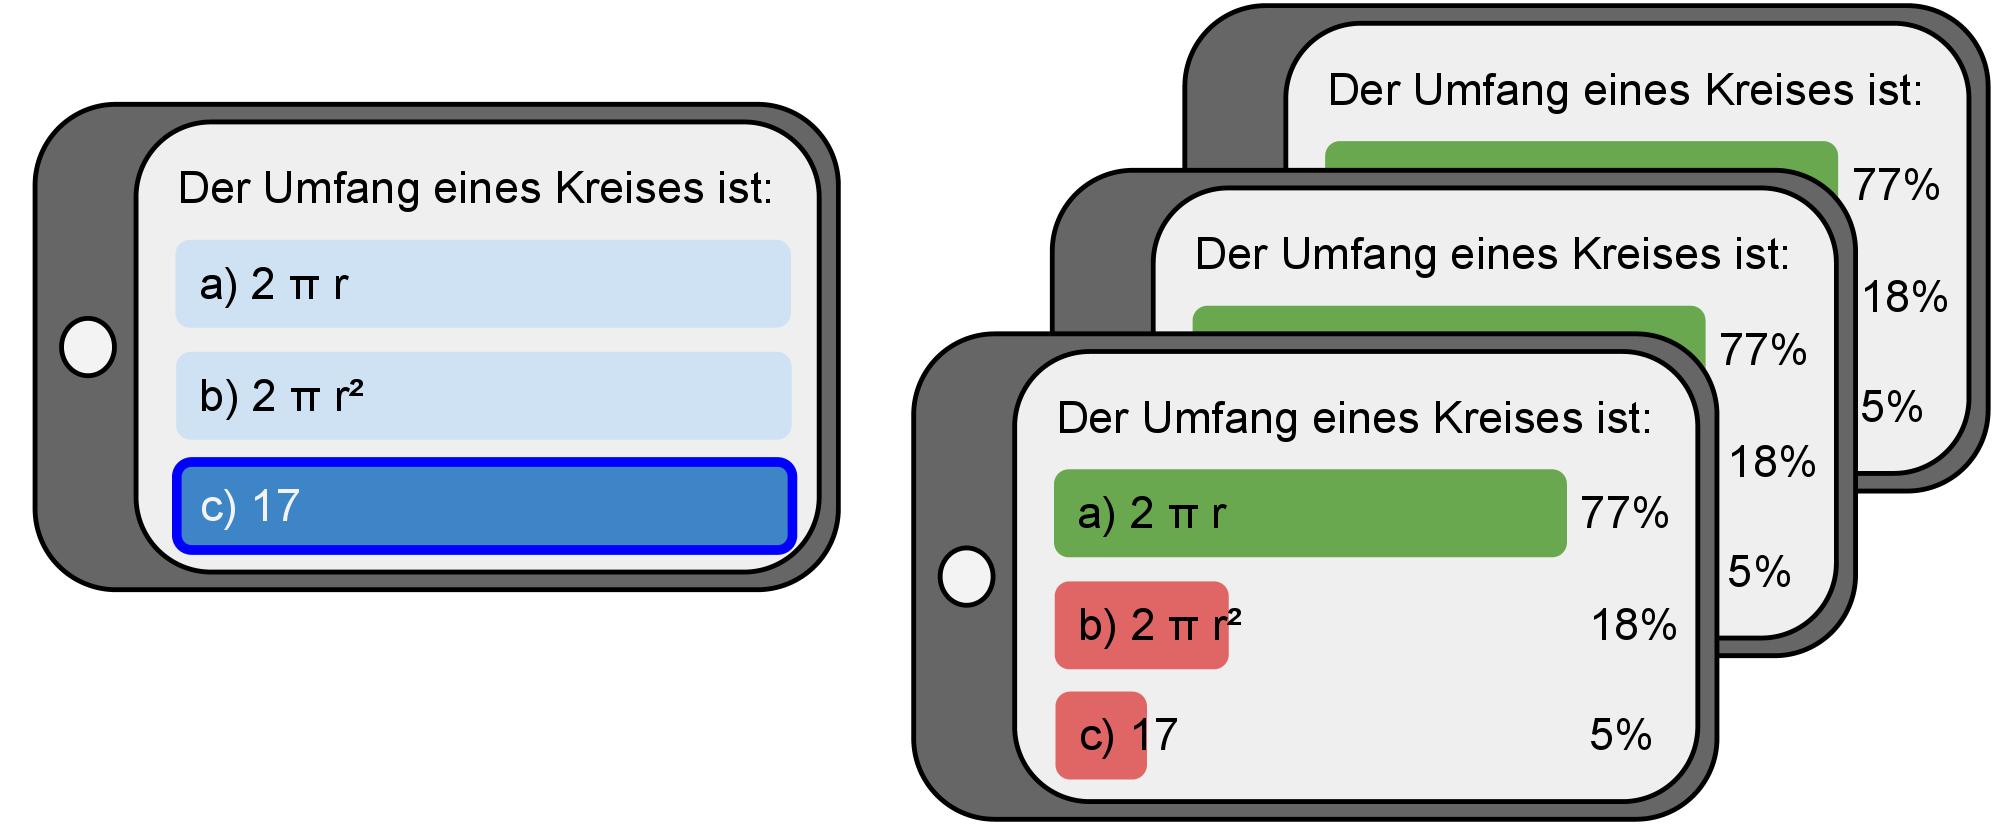
\includegraphics[width=0.75\textwidth]{media/Umfrage.png}
\end{center}
\caption{Eine einfache Umfrage}
\label{f:umfrage}
\end{figure}

Abbildung~\ref{f:umfrage} zeigt schematisch die Darstellung einer Umfrage. In der Anwendung sind insgesamt drei Arten von Umfragen möglich: bei \emph{Einfach-Auswahl-Fragen} muss genau eine Antwort ausgewählt werden, bei \emph{Mehrfach-Auswahl-Fragen} muss eine oder mehrere Antworten ausgewählt werden und bei \emph{Wert-Eingaben} wird als Antwort eine Zahl erwartet, wobei der Fragesteller den möglichen Wertebereich einschränken kann. Mit diesen Frage-Typen ist es möglich beliebige andere Gruppenbefragungen durchzuführen. Abbildung~\ref{f:fotoabstimmung} zeigt schematisch den Einsatz der Anwendung in einer Foto-Abstimmung. Die Teilnehmer der Gruppe können mit ihren Mobilgeräten Fotos machen oder vom Gerät auswählen und zur Abstimmung stellen. Die Fotos werden in der Gruppe verteilt und bei der Abstimmung kann jeder Teilnehmer alle Fotos auf seinem Gerät betrachten und bewerten.

\begin{figure}[htb]
\begin{center}
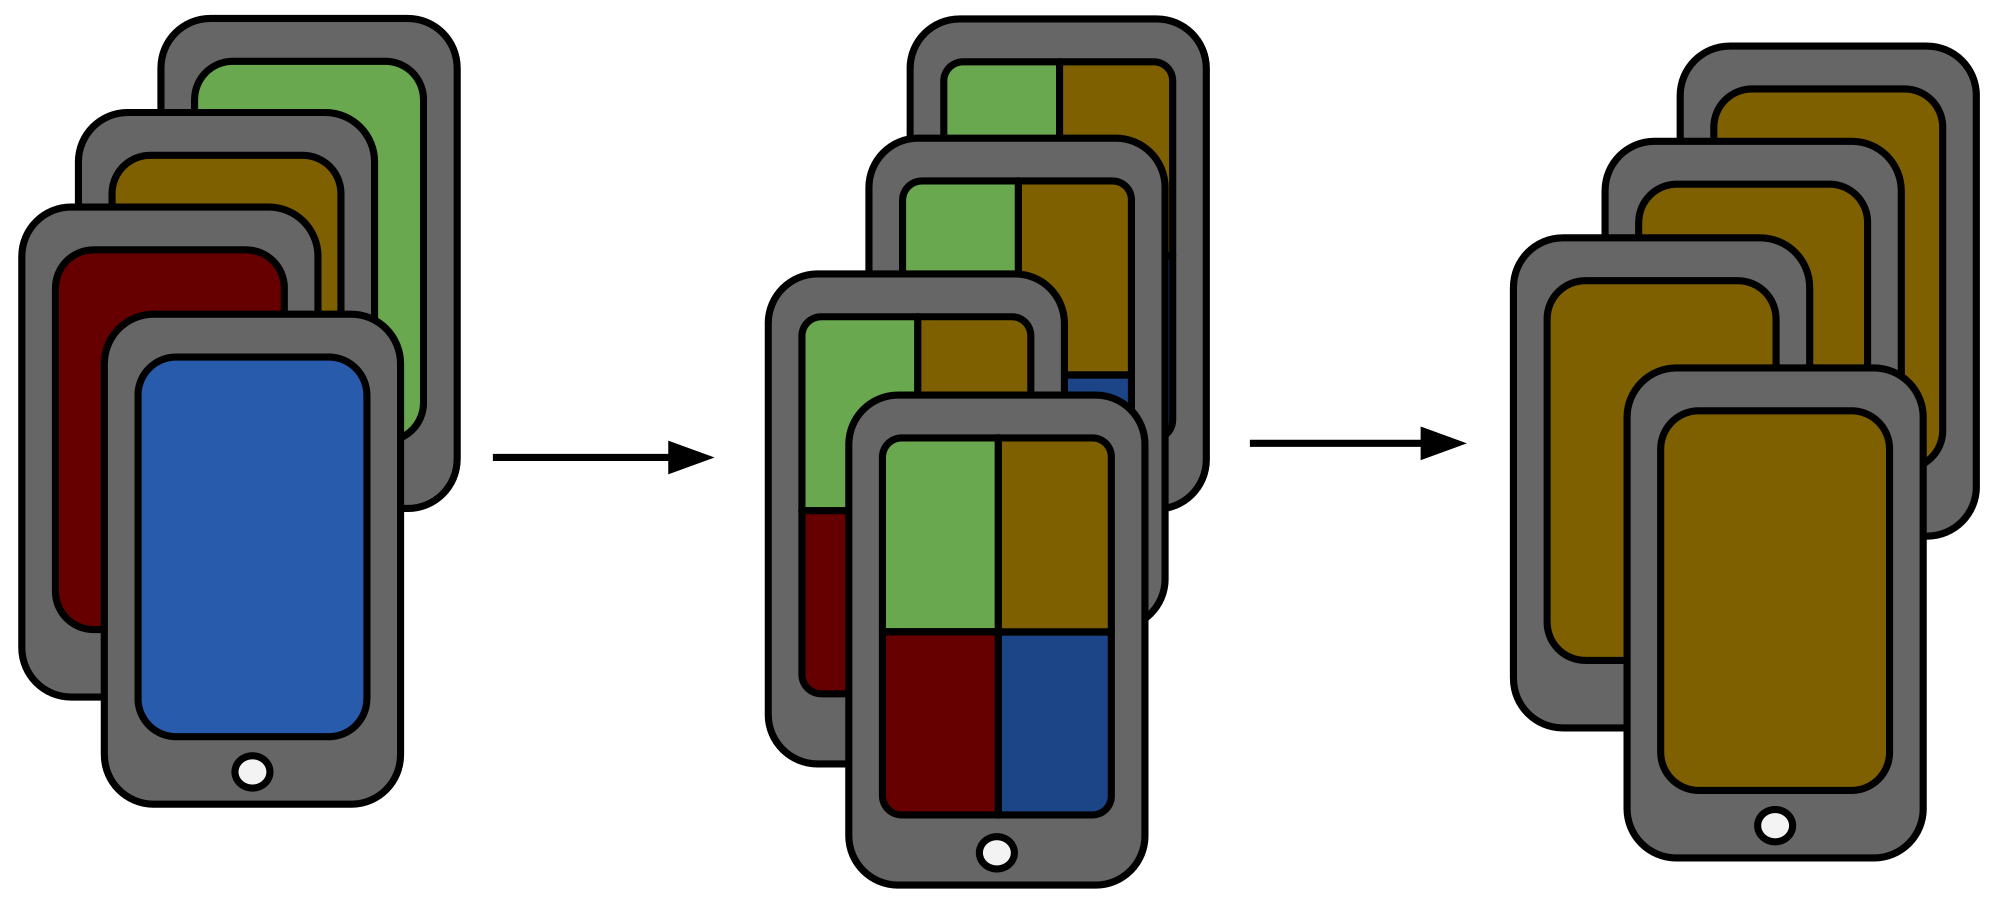
\includegraphics[width=0.75\textwidth]{media/Fotoabstimmung.png}
\end{center}
\caption{Foto-Abstimmung}
\label{f:fotoabstimmung} 
\end{figure}


\section{Aufbau der Anwendung}

Aus den im vorigen Abschnitt genannten Funktionen lassen sich die folgenden Anforderungen an die Anwendung ableiten: Es muss möglich sein, Veranstaltungen anzulegen und zu diesen Veranstaltungen wiederum Fragen, die von Teilnehmern dieser Veranstaltung beantwortet werden können. Das Antworten soll dabei während der Veranstaltung möglich sein, die Auswertung der Ergebnisse während und nach der Veranstaltung. Die Fragen müssen in eine zeitliche Reihenfolge gebracht werden können. Zur Bewertung der Präsentation sollten deren Folien in der Anwendung verfügbar sein. Zusätzlich ist es wünschenswert auch freie Kommentare zu Veranstaltungen zu erhalten, die Teilnehmer können so z.B. auf Fehler in einer Präsentation hinweisen oder unklare Aspekte aufzeigen.

\subsection{Datenmodell}

\begin{figure}[htb]
\begin{center}
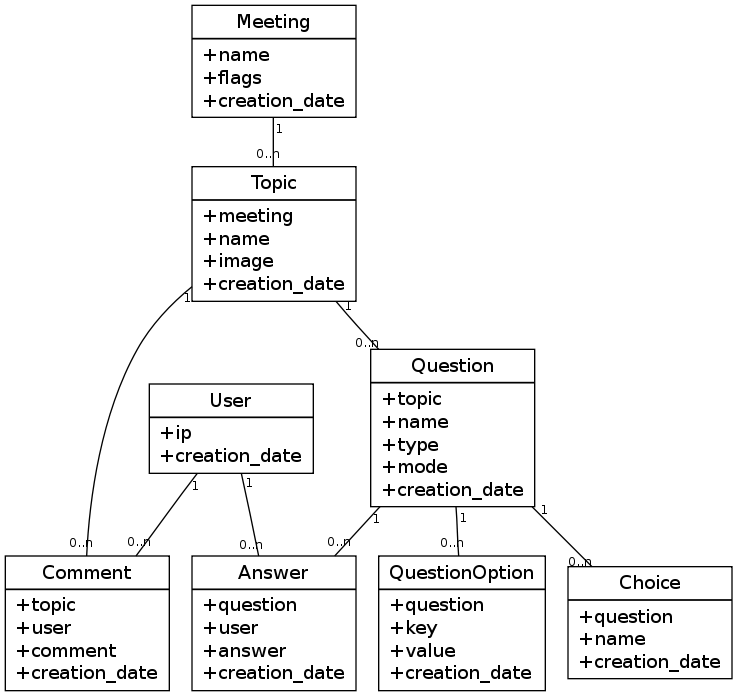
\includegraphics[width=0.75\textwidth]{media/models.png}
\end{center}
\caption{Datenmodell der Anwendung}
\label{f:models}
\end{figure}

\emph{GroupMood} wurde so entwickelt, dass, in einem gewissen Rahmen, beliebige Anwendungsfälle abgebildet werden können. Abbildung~\ref{f:models} zeigt das zugrundeliegende Datenmodell. Die Basis bildet hierbei immer ein \emph{Meeting}, also ein Zusammentreffen von mehreren Personen. Im Verlauf dieses Meetings können verschiedene Arten von Fragen (\emph{Question}) gestellt werden, wobei eigentlich nur zwei Arten von Fragen auftreten. Bei \emph{Von-Bis-Fragen} wählt der Teilnehmer die Antwort auf einem vorgegebenen Zahlenbereich aus. Es kann sich dabei um eine Jahreszahl handeln, z.B. "`Wann ist Napoleon gestorben? Wählen Sie zwischen 1800 und 1900"' oder auch um die Frage nach einer Bewertung "`Wie gut hat ihnen diese Veranstaltung gefallen? Wählen Sie auf einer Skala von 1 bis 10"'. Bei \emph{Auswahl-Fragen} ist der Freiheitsgrad soweit eingeschränkt, dass die Antwort aus einer Auswahl von Antwortmöglichkeiten (\emph{Choice}) ausgewählt werden muss, z.B. "`Wie heißt der aktuelle Bundespräsident? Johannes Rau, Horst Köhler oder Christian Wulff"'. Bei diesem Typ ist es üblich auch mehrere Antwortmöglichkeiten zu zu lassen, z.B. "`Albert Einstein war: Deutscher, vom Sternzeichen Löwe, Physiker. Wählen Sie alle korrekten Antworten"'.

Wie oft eine Antwort pro Teilnehmer dabei abgegeben werden kann, lässt sich ebenfalls mit nur zwei Fällen umfassend beschreiben. So können Antworten entweder einmal pro Frage und Teilnehmern abgegeben werden, oder ständig. Mit der Möglichkeit die Antwort ständig zu ändern kann z.B. die laufende Bewertung eines Meetings abgebildet werden, bei der die Teilnehmer während des Meetings ihre Bewertung jederzeit anpassen können. Tabelle~\ref{table:questiontypes} liefert eine Übersicht über die möglichen Fragetypen und die jeweiligen Einstellungen mit denen diese konfiguriert werden.

Um Fragen im Verlauf einer Veranstaltung passend anzeigen zu können, müssen diese in eine Reihenfolge gebracht werden können. Die Reihenfolge der Fragen wird dabei mit Hilfe von Themen (\emph{Topic}) gruppiert. Ein Thema kann dabei das gesamte Meeting, aber auch eine einzelne Präsentationsfolie sein. So ist es möglich den Ablauf der einzelnen Fragen flexibel fest zu legen und an den jeweiligen Anwendungsfall an zu passen. Zusätzlich ist es möglich, einem Thema ein Bild zu zuweisen, so dass hierüber die Bewertung von Folien einer Präsentation möglich ist.

Neben der Fragen gibt es mit Freitext-Kommentare (\emph{Comment}) eine weitere Möglichkeit, Feedback zu hinterlassen. Kommentare werden dabei wie die Fragen immer zu Themen abgegeben.

Mithilfe von Zusatzinformationen (\emph{Flags}), die auf dem Meeting gesetzt werden können, ist es möglich das Verhalten der Anwendung anzupassen. Ist z.B. das Flag \texttt{fotovote} gesetzt, wird signalisiert, dass es sich bei dem Meeting um eine Foto-Abstimmung handelt. Dadurch ist es serverseitig möglich, neue Themen anzulegen, wobei ein Thema einem Foto entspricht. Zu jedem Thema wird automatisch eine Wertebereichs-Frage zur Bewertung des Fotos angelegt. In der App werden bei diesen Meetings zusätzliche UI-Elemente angezeigt, die es den Teilnehmern der Foto-Abstimmung ermöglichen, direkt aus der App weitere Fotos hinzuzufügen.

\begin{table}
\begin{center}
\begin{tabular}{l l l c c c c}
& & & \multicolumn{4}{c}{QuestionOption} \\
& \multicolumn{2}{c}{Question} & \multicolumn{2}{c}{Anzahl Optionen} & \multicolumn{2}{c}{Wertebereich} \\
Frage-Typ & type & mode & min & max & min & max \\
\hline
Single-Choice & choice & single & 1 & 1 & --- & --- \\
Multiple-Choice & choice & single & $\geq$1 & $\geq$min & --- & --- \\
Wert-Auswahl & range & single & --- & --- & $\geq$0 & >min \\
Bewertung & range & average & --- & --- & $\geq$0 & >min \\
\end{tabular}
\caption{Mögliche Fragen und deren Konfiguration}
\label{table:questiontypes}
\end{center}
\end{table}

\subsection{Umsetzung}

\begin{figure}[htb]
\begin{center}
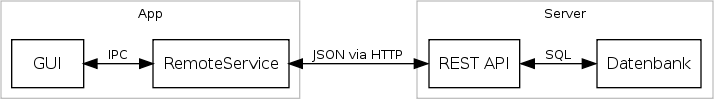
\includegraphics[width=\textwidth]{media/system.png}
\end{center}
\caption{Aufbau des Systems}
\label{f:system}
\end{figure}

Mit \emph{GroupMood} sollen vielen Teilnehmer gleichzeitig an Umfragen teilnehmen können. Um die theoretisch sehr große Anzahl gleichzeitiger Anfragen performant verarbeiten zu können, findet die Kommunikation zwischen den einzelnen Teilnehmern über einen Server auf Django\footnote{\url{https://www.djangoproject.com/}}-Basis statt. Dort werden auch die erzeugten Daten in einer Datenbank gespeichert. Die App greift auf diese Daten über eine \emph{RESTful} HTTP-Schnittstelle zu. Um eine saubere Trennung zwischen GUI-Code und dem Zugriff auf den Server zu erreichen findet jegliche Kommunikation in einem \emph{RemoteService} statt, der von den einzelnen \emph{Activities} der App gebunden wird. In Abbildung~\ref{f:system}  ist der Aufbau des Systems schematisch dargestellt. Die App ist dabei nicht an die Verwendung eines bestimmten Servers gebunden -- sie akzeptiert URLs mit dem Protokoll \texttt{grpmd}, bzw. \texttt{grpmd+ssl} und verwendet diese, um daraus die HTTP(S)-URL zum Server zu generieren (siehe Tabelle~\ref{table:urlschema}).

\begin{table}[htb]
\begin{center}
\begin{tabular}{l l}
\emph{GroupMood}-URL & Server-URL \\
\hline
\texttt{grpmd://<host>/<id>} & \texttt{http://<host>/groupmood/meeting/<id>} \\
\texttt{grpmd+ssl://<host>/<id>} & \texttt{https://<host>/groupmood/meeting/<id>} \\
\end{tabular}
\caption{Umwandlung \emph{GroupMood}-URL in Server-URL}
\label{table:urlschema}
\end{center}
\end{table}

Um die Serialisierung und Deserialisierung zu vereinfachen verwendet das Datenformat JSON-LD\footnote{http://json-ld.org/} hierbei werden die JSON-Daten mit Informationen zum Kontext angereichert, so dass der Verwender erkennen kann, wie die Daten zu interpretieren sind. In der App werden diese Informationen verwendet, um aus den JSON-Daten automatisch die passenden Models erzeugen zu können.

\subsection{Verwendung}

Um an die Daten eines Meetings zu gelangen benötigt die Anwendung eine URL, unter der sie die Daten laden kann. Diese kann z.B. über einen QR-Code übermittelt werden, es ist aber auch möglich, URLs direkt aus Benachrichtigungen oder aus dem Browser zu öffnen. Sind die Daten des Meetings geladen, kann der Benutzer zwischen den einzelnen Themen navigieren. Hierbei sieht er den Namen des Themas oder, falls vorhanden, eine kleine Vorschau der hinterlegten Folie. Die Bilder werden dabei durch den Service im Hintergrund nachgeladen, so kann der Nutzer schnell alle anderen Funktionen der Anwendung verwenden. Die Folienansicht kann auf Vollbildansicht umgeschaltet werden, in der das Bild in höherer Auflösung angezeigt wird, so dass man alle Details der Folie erkennen kann. Zu jedem Thema werden die hinterlegten Fragen angezeigt, durch die mittels einer Wischgeste schnell durchgeblättert werden kann. Je nach Frage-Typ wird ein Werte-Slider oder eine Options-Auswahl angezeigt. Über drei Icons im oberen Bereich des Anwendungsfensters kann zwischen der Darstellung der Fragen, den Kommentaren zu den Fragen und den kumulierten Antworten der Gruppe hin und hergeschaltet werden.

\subsection{GUI-Konzept}

\begin{figure}[htb]
\begin{center}
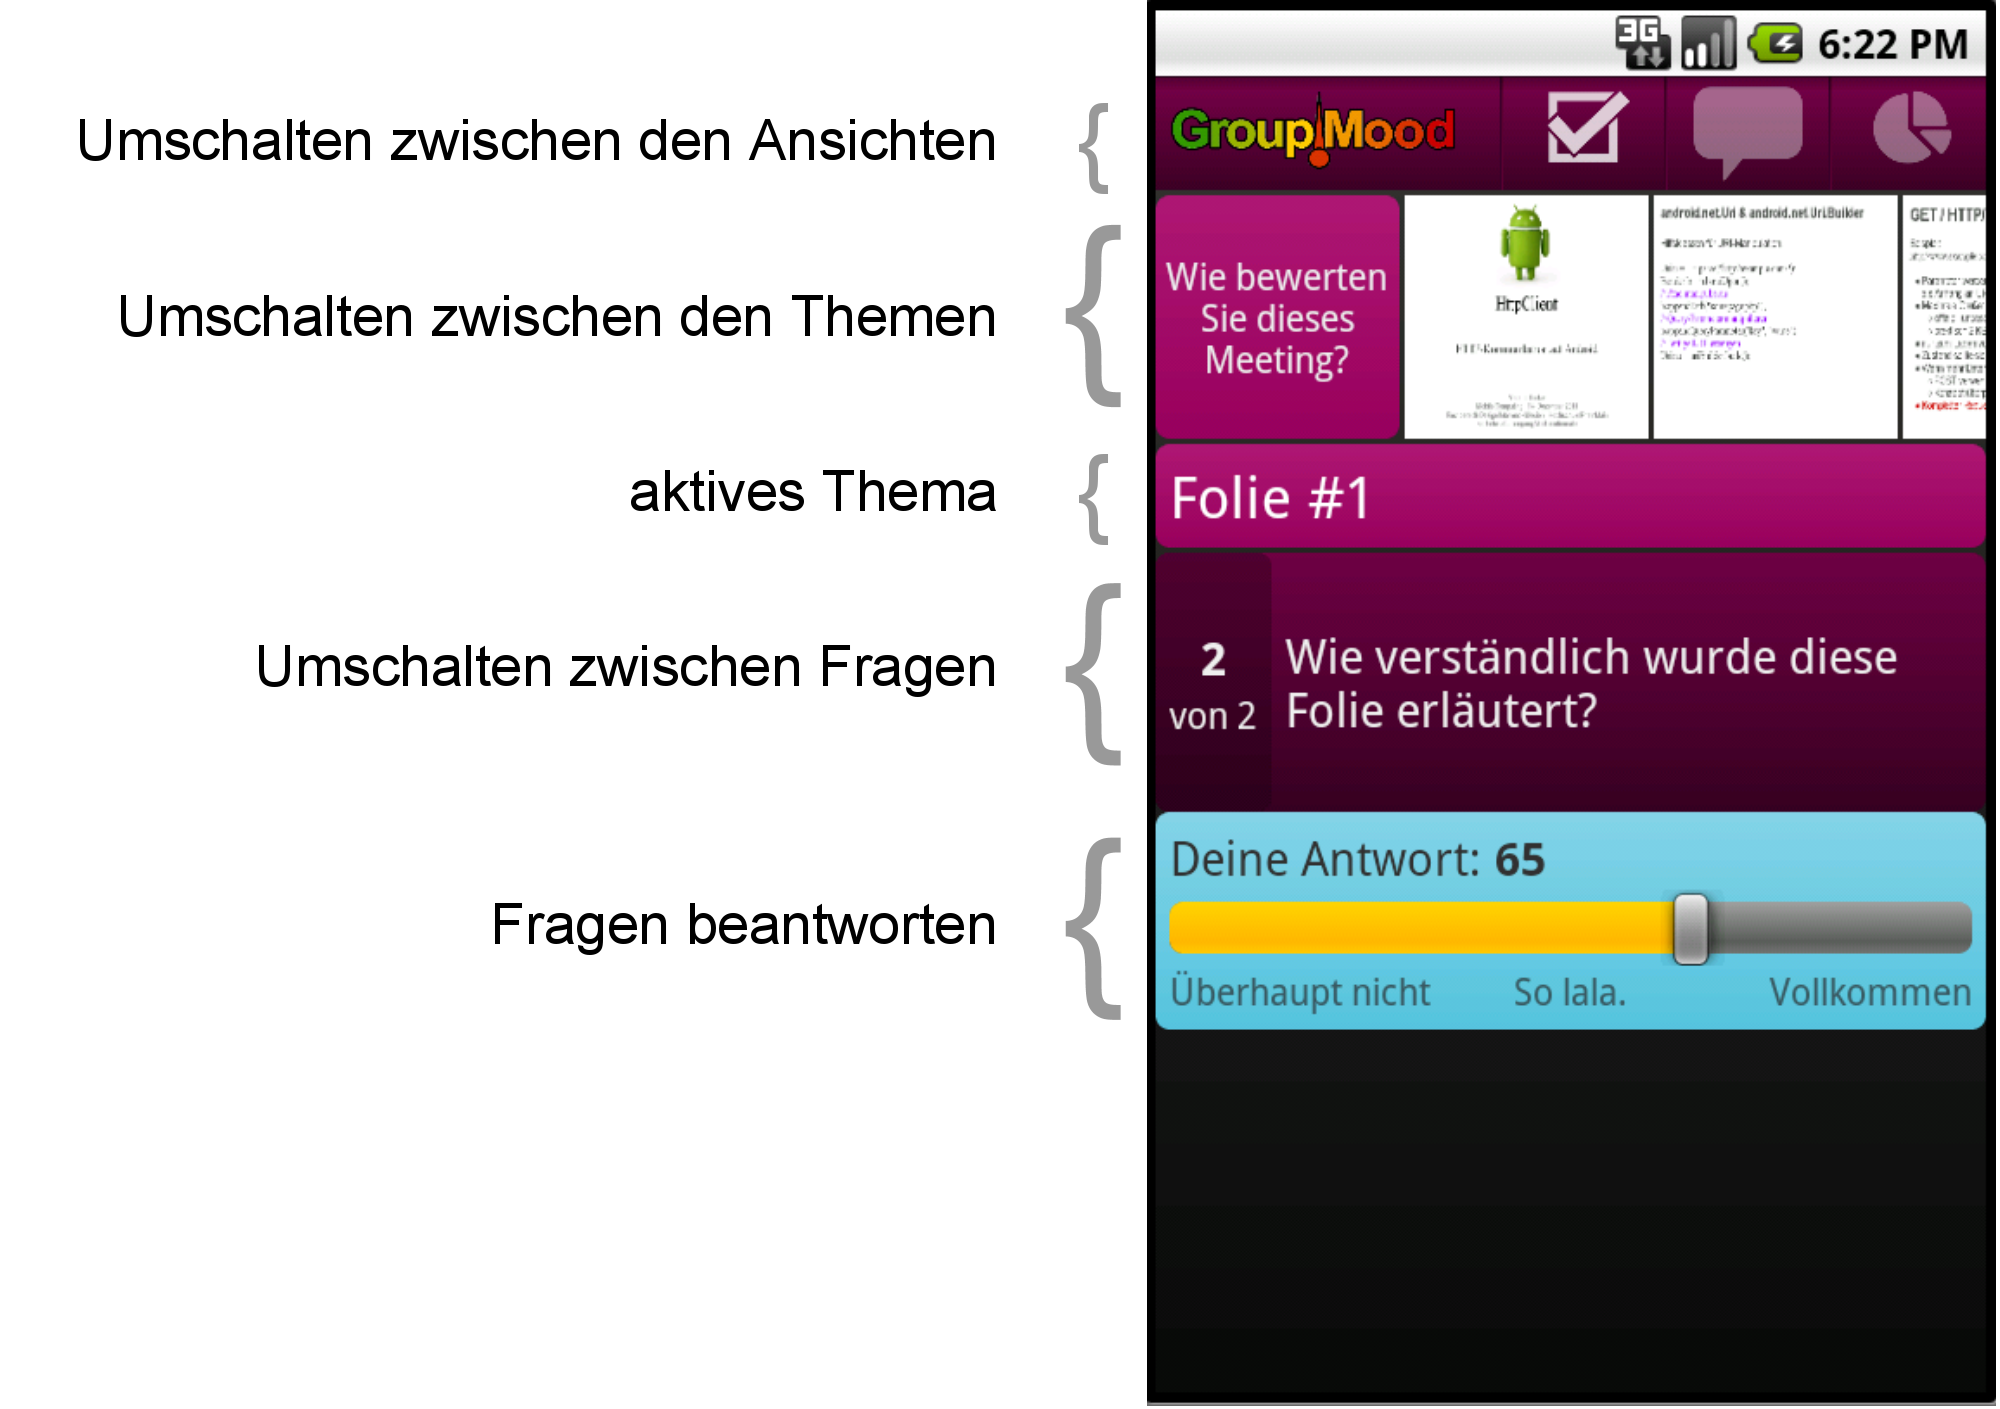
\includegraphics[width=\textwidth]{media/app.png}
\end{center}
\caption{GUI der App}
\label{f:gui}
\end{figure}

Abbildung~\ref{f:gui} zeigt die App in der Darstellung, in der Fragen beantwortet werden. Bei der Gestaltung der App wurde versucht, eine möglichst einfache Bedienung zu ermöglichen -- der Teilnehmer soll nicht von der Veranstaltung abgelenkt werden und schnell die gewünschte Aktion ausführen können. Um dieses Ziel zu erreichen, wurde weitestgehend auf eigene Bedienelemente verzichtet und nur die nativen GUI-Elemente verwendet. Das Navigieren zwischen den einzelnen Themen und deren Fragen erfolgt mit Hilfe einfacher horizontaler und vertikaler Wischgesten, die dem Nutzer allgemein als "`scrollen"' bekannt sind. Um die einfache Orientierung zu unterstützen werden die einzelnen Bereiche der Anwendung farblich unterschieden: informelle Bereiche sind in einem sanften lila gehalten, während die Bereiche, in denen der vom Benutzer Eingaben erwartet werden in einem kräftigen Cyan dargestellt werden.

\end{document}
